% !TEX root = ../MemPod.tex
\section{Results}
\label{sec:Results}

\subsection{Evaluation Framework}
\label{sub:Evaluation}

The goal of our evaluation framework is to quantitatively and qualitatively assess MemPod's capabilities and compare it against state-of-the-art proposed mechanisms. Throughout our evaluation section, we study MemPod's performance running as part of an eight-core CPU. We extended Ramulator \cite{kim-ramulator} to support flat address space hybrid memories and with MemPod for our memory simulations. HMA and THM were also implemented in our simulation framework for comparison purposes. Ramulator allows for cycle-level memory simulation and includes a simple CPU front-end capable of approximating resource-induced stalls. We chose to evaluate MemPod under a realistic memory configuration consisting of 1GB 3D-stacked HBM \cite{JEDEC-HBM-REVISED} and 8GB of off-chip DDR4-1600. Table \ref{tab:specs} Provides a more detailed description of the simulated system's configuration.

\begin{table}[t]
  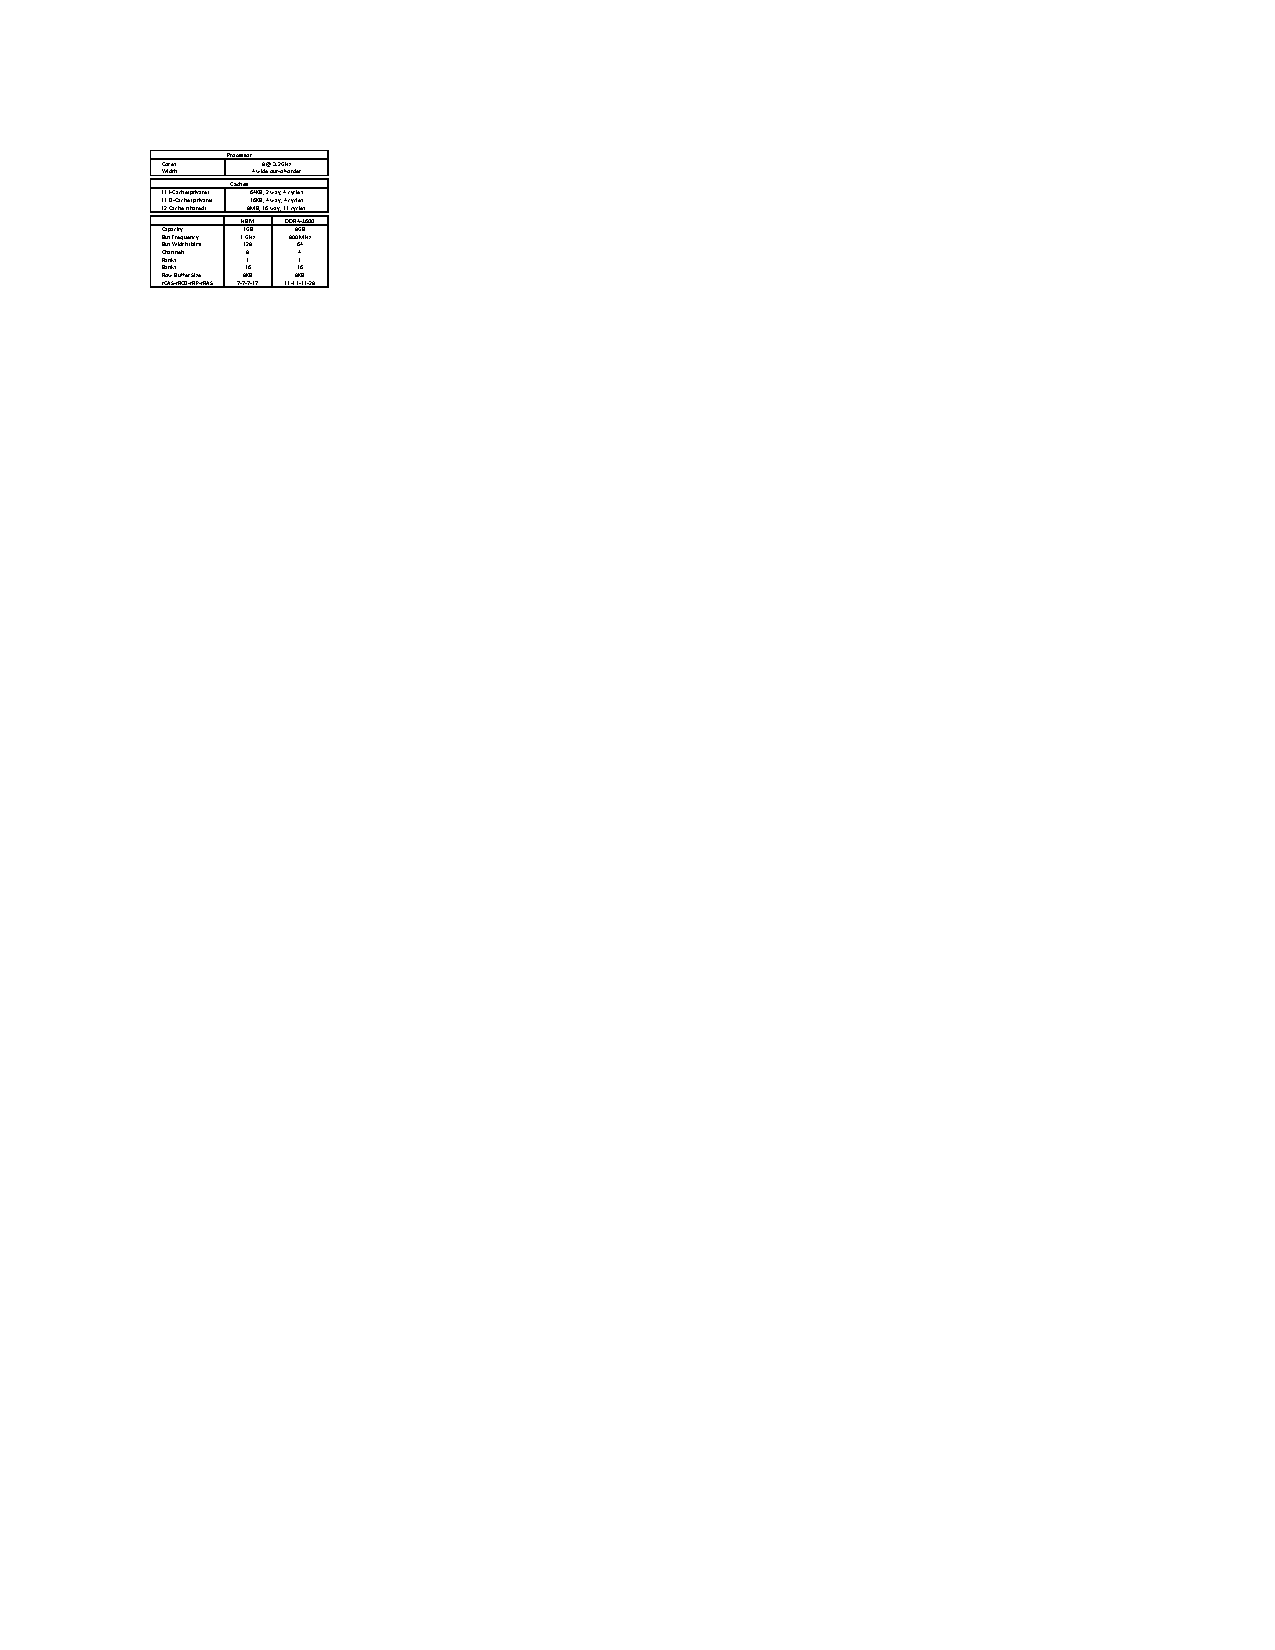
\includegraphics[width=0.46\textwidth]{figures/specs_table.pdf}
  \caption{Experimental framework configuration}
  \label{tab:specs}
\end{table}

\subsection{Experimental Methodology}
\label{sub:Experimental}

We used benchmarks from the SPEC2006 suite \cite{spec} as our workloads. Using Sniper \cite{sniper}, we recorded memory request traces while simultaneously executing 8 benchmarks on a simulated 8-core CPU. We then feed these multi-programmed memory traces in Ramulator, executing all workloads to completion. Our complete set of workloads consists of 16 ``homogeneous'' workloads, where the same benchmark runs 8 times in parallel (we simply call this workload with the benchmark's name in later results), as well as 12 workloads featuring a random mix of 8 benchmarks each (marked as mix1-12). A breakdown of the mixed workloads is shown in Table \ref{tab:workloads}.


We also extended Ramulator with caches needed for activity tracking and/or remap tables depending on the simulated mechanism. Cache misses inject a memory request into the stream of requests fed by our trace files to retrieve the missing information. No priority is given to cache miss requests over the rest of the requests. When caches are disabled, the simulator assumes that any information needed by any mechanism exists on chip and is accessible without any delay. The migration process was implemented in detail as well. In order to read an entire 2KB page from memory, 32 read requests need to be sent for each of the two migration candidates and then another set of 32 requests for each of the two write-backs.

Since we used Ramulator with recorded traces, we chose to report Average Main Memory Time in our results instead of IPC. Even though Ramulator has the ability to approximate IPC, AMMT is a more accurate metric since it models the memory in detail. AMMT is the average time spent in main memory by each request (lower is better). Due to space limitation we are not able to show results from all our workloads in most of the graphs in this paper. In those graphs, we only present the average of all mixed workloads, average of all homogeneous workloads and overall average.

\begin{table}
  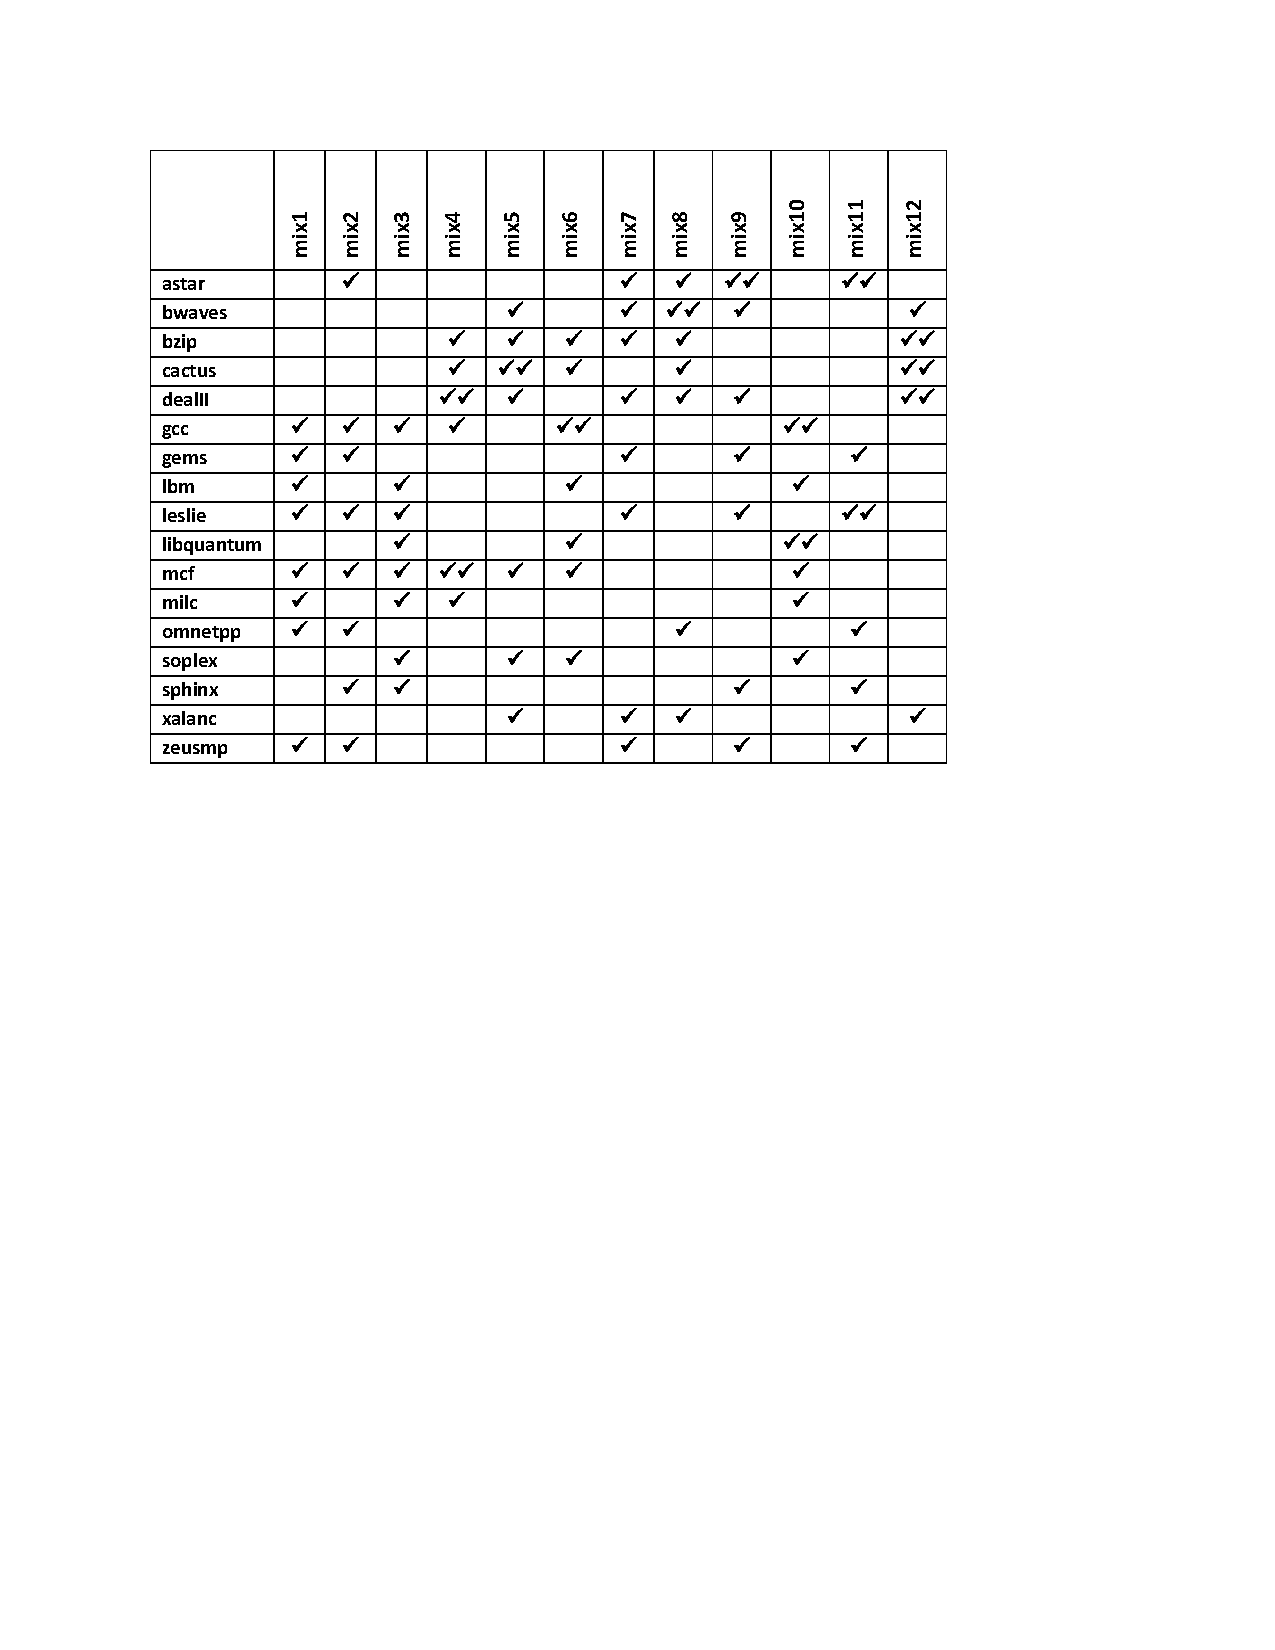
\includegraphics[width=0.46\textwidth]{figures/workloads_checkmarks.pdf}
  \caption{Mixed workloads description}
  \label{tab:workloads}
\end{table}

\subsection{Simulation Results}
\label{sub:SimResults}

\subsubsection{Optimal Parameter Values}

MemPod exposes 3 variables that allow fine-tuning it based on a particular system or expected workloads: (1) The number of MEA counters, (2) interval length and (3) the size of each MEA counter. Identifying the optimal values for each parameter can maximize MemPod's capabilities. The number of MEA counters dictates the highest possible number of migrations that can be performed at each interval, while the epoch length will determine MemPod's ability to better adapt to phase changes in a workload. The size of each MEA counter can affect performance due to the loss of information when smaller counters are used but can also save space on the chip.

We first identified the optimal number of MEA counters, by keeping the epoch length constant and exponentially increasing the number of counters from 16 to 512. In order to minimize the impact of other factors, we executed this experiment with 16 bits per counter and caches disabled. In other words, each counter was given more than enough space and all required information such as the remap table resides entirely on the chip and is accessible at no cost. 

Figure \ref{fig:num_counters} shows Average Main Memory Time (AMMT) normalized over the AMMT when 16 counters are used, along with the average number of migrations per Pod per epoch (secondary axis). The results indicate that each Pod utilizes the higher number of counters and consecutively performs more migrations per interval, however performance is degraded when more than 128 counters were used. Using 128 counter, AMMT is improved by 6\% over the baseline with 16 MEA counters. 

\begin{figure}[h]
	\centering
  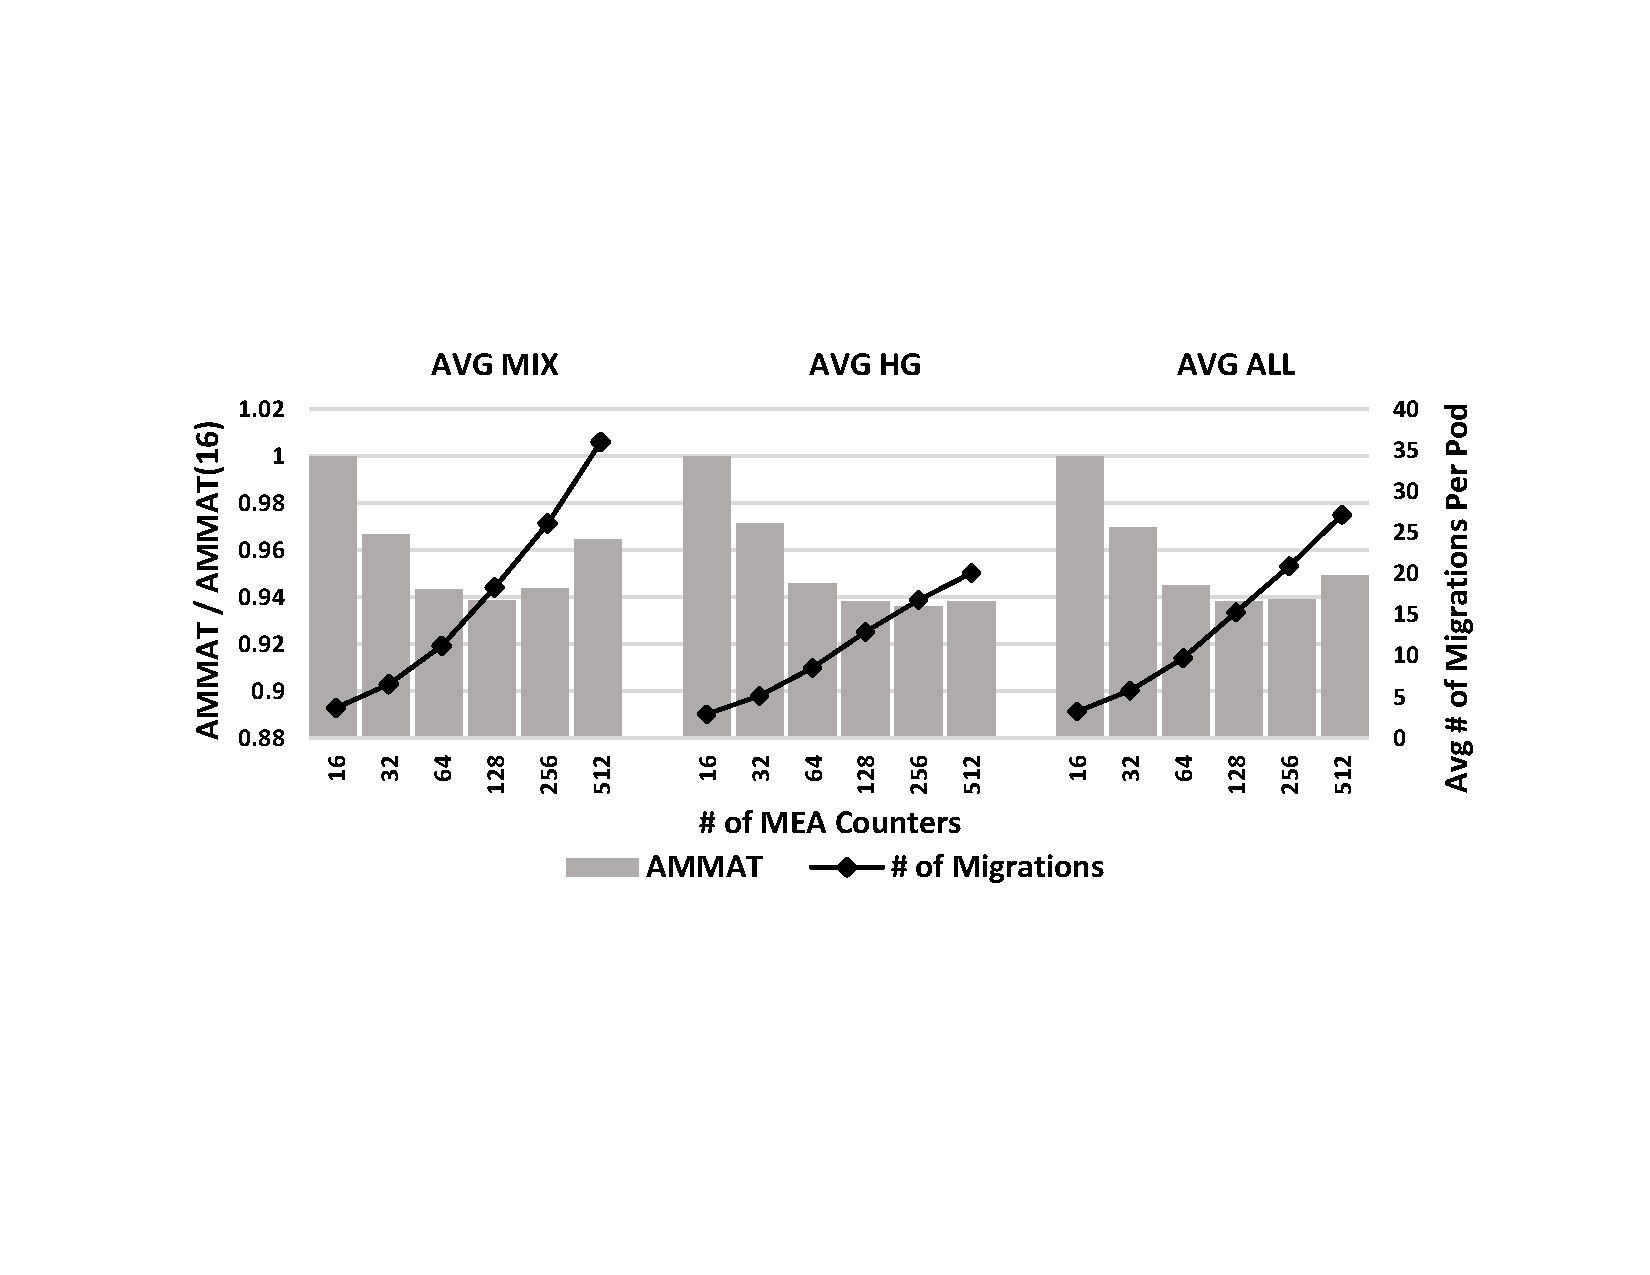
\includegraphics[width=0.46\textwidth]{figures/avg_num_counters_normalized.pdf}
  \caption{\# of MEA Counters Vs Normalized AMMT (primary axis) and average \# of Migrations per Pod per interval (secondary axis)}
  \label{fig:num_counters}
\end{figure}

After identifying the optimal counter number, Figure \ref{fig:interval} displays the same measurements as Figure \ref{fig:num_counters} with a varying epoch length. Caches were again disabled, each counter was given 16 bits and the number of MEA counters was set to the optimal value of 128. We observe that on average, MemPod reports the lowest AMMT with interval length of 100$\mu$s (2\% improvement over 50 $\mu$s on average). As the interval length increases, more migrations are performed and AMMT increases. Dropping below 100$\mu$s has a negative effect on AMMT. For comparison purposes, HMA \cite{meswani-HPCA21} identified the optimal epoch length to be 1ms (10x larger) in order to support all lengthy processes that take place during a migration event.

\begin{figure}[h]
  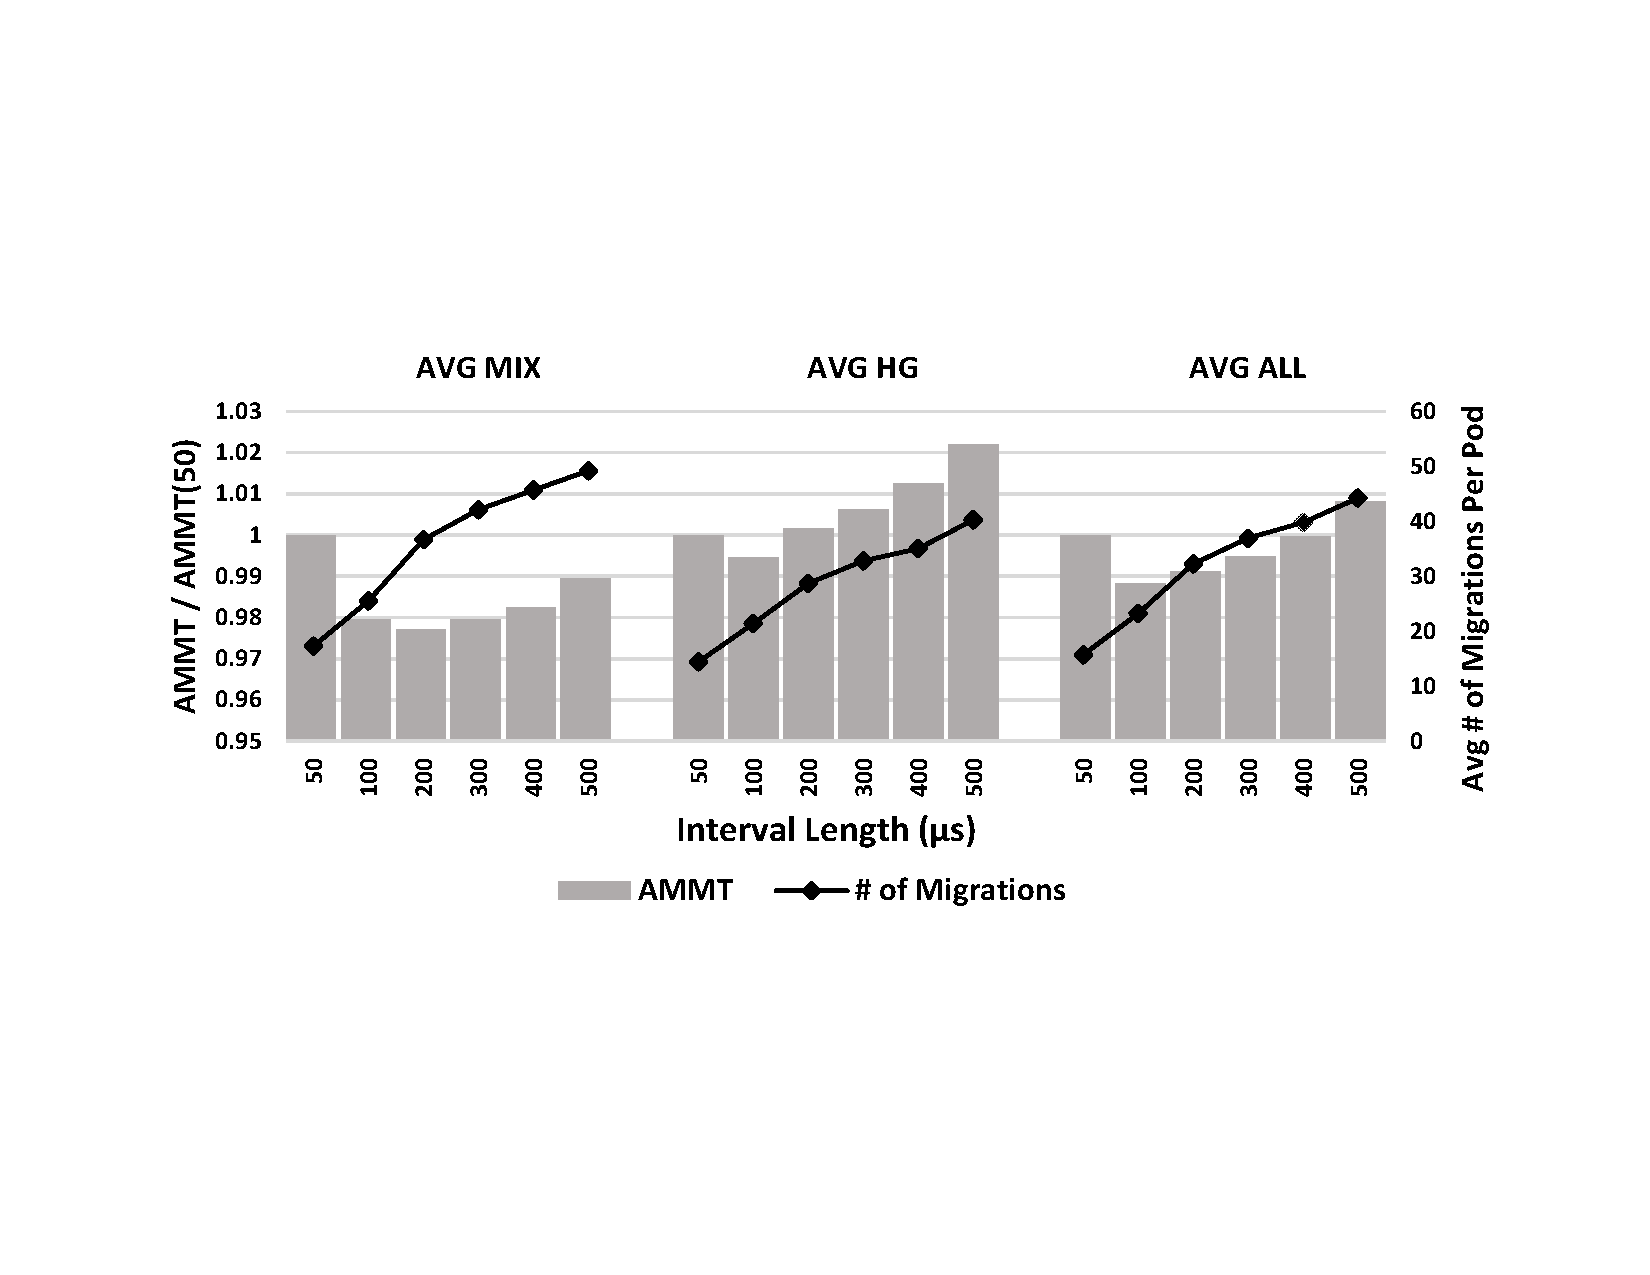
\includegraphics[width=0.46\textwidth]{figures/interval_length_normalized.pdf}
  \caption{Interval Length Vs Normalized AMMT (primary axis) and average \# of Migrations per Pod per interval (secondary axis)}
  \label{fig:interval}
\end{figure}

As previously explained in Section \ref{sec:MEA}, the MEA algorithm cannot be cached efficiently and as a result, the entire activity tracking structure needs to be on chip. The size (in bits) of each counter defines the area requirements of our MEA tracking mechanism. We modified the MEA algorithm to remove map entries with counter values equal to or less than zero (instead of strictly equal to zero) in order to support counter saturation. We opted not to immediately remove an overflowed counter even though its value is now zero, since the existence of the correct counter set is crucial to the algorithm's accuracy. For this experiment we used the optimal parameter values identified in the previous experiments and set the number of MEA counters to 128 and interval length to 100us. All caching was disabled in order to study the direct impact of this variable.

Figure \ref{fig:counter_size} presents the impact of counter size on AMMT and average number of migrations. We first observe that 8 bits are sufficient for our workloads, since larger sizes report identical results. Our second observation is that two bit counters report a negligible performance degradation (0.3\% on average) over 8 bit counters and a reduced average number of migrations.

\begin{figure}[h]
  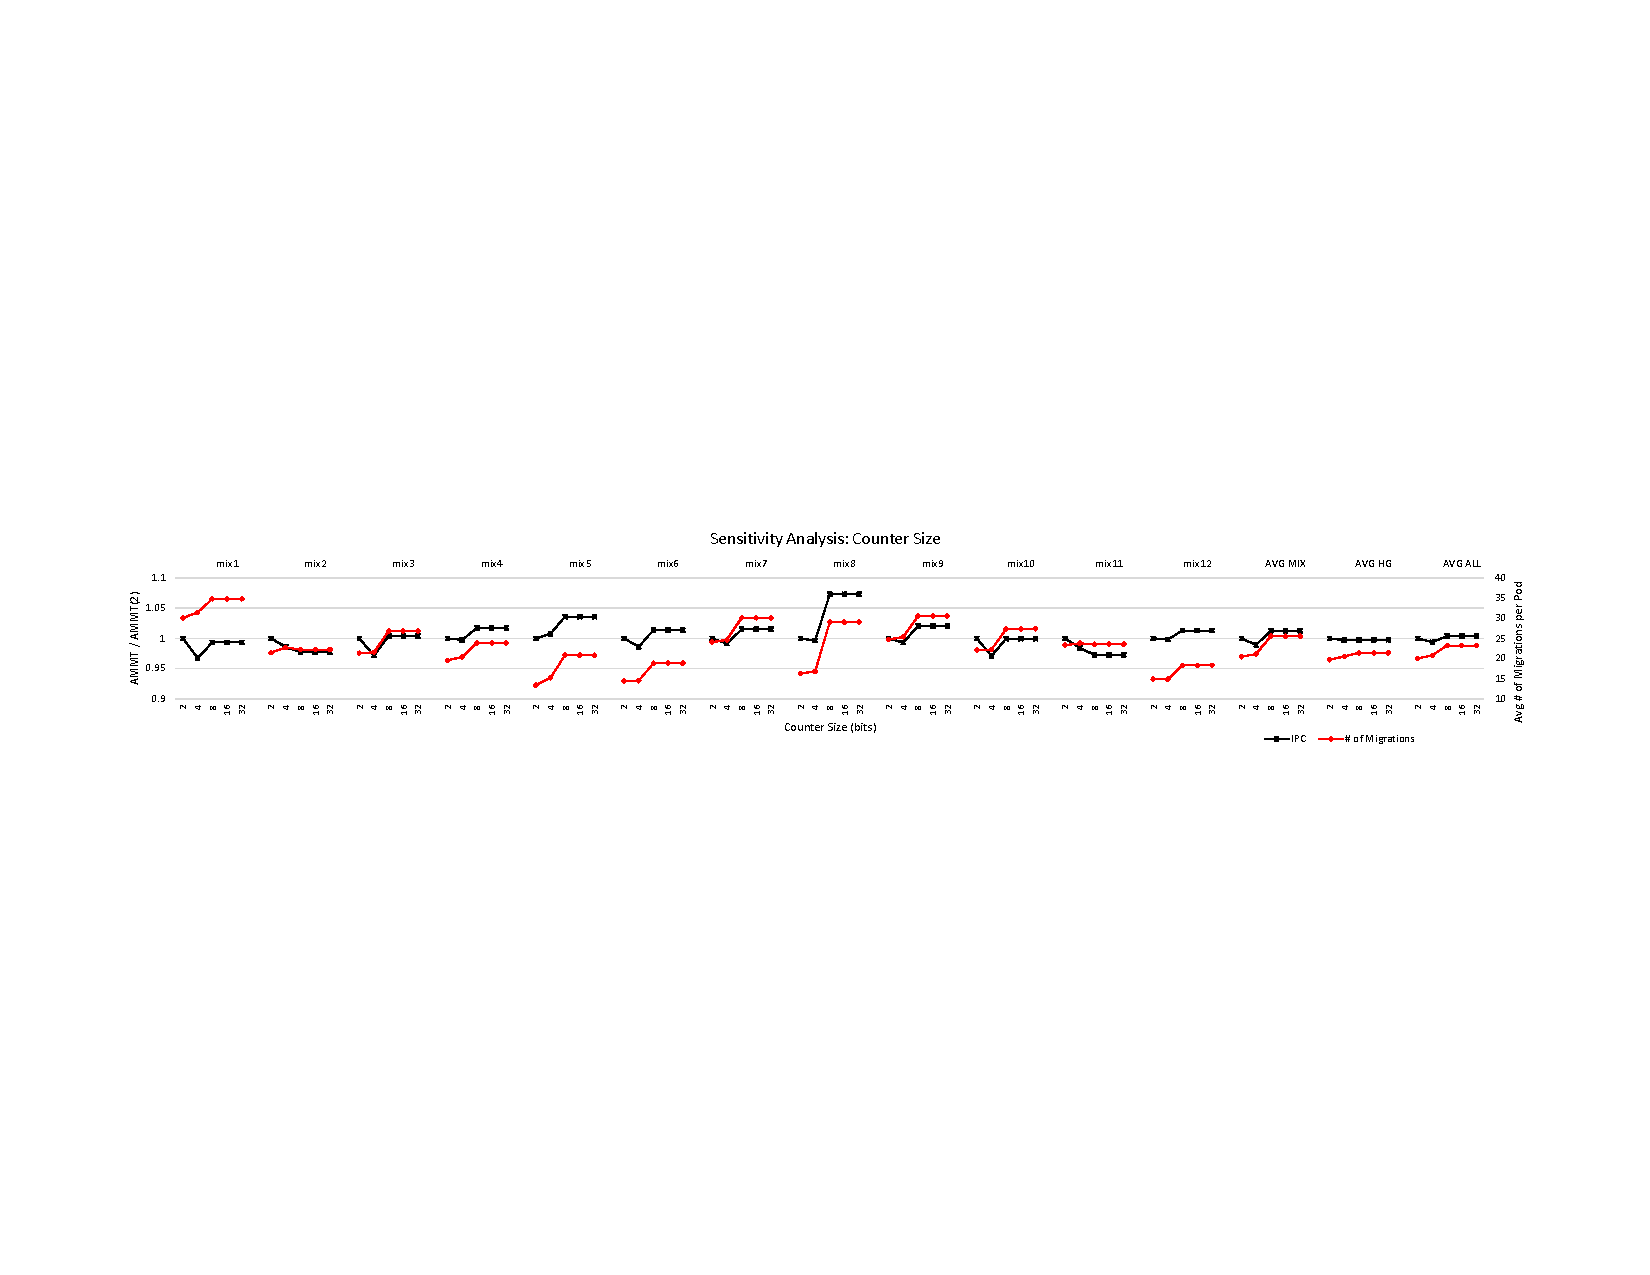
\includegraphics[width=0.46\textwidth]{figures/counter_size_normalized.pdf}
  \caption{Counter size (in bits) Vs Normalized AMMT (primary axis) and average \# of Migrations per Pod per interval (secondary axis)}
  \label{fig:counter_size}
\end{figure}

The most interesting observation comes from assigning 4 bits to each counter. On average, performance is boosted slightly (up to 3\% and 0.6\% on average) even compared to using larger counters, while migration count is low. %Since a difference is observed, we can conclude that these smaller counters ``lose'' information that in turn benefits overall execution. The reported result is a welcomed artifact of the MEA algorithm combined with application behavior. 

Based on our results, we identify 4 bits per counter to be the optimal value. Each one of the 128 MEA entries needs 21 bits for addressing the 1125K pages per Pod and 4 bits for its counter, leading to an area cost of only 400B per Pod and $\sim$1.5KB total. Compared to the state of the art, MemPod's activity tracking requirement is $\sim$341x smaller than THM's (512KB) and $\sim$6100x smaller than HMA's (9MB).


\subsubsection{Performance Comparison}
\label{sub:performance}

\begin{figure*}[t]
  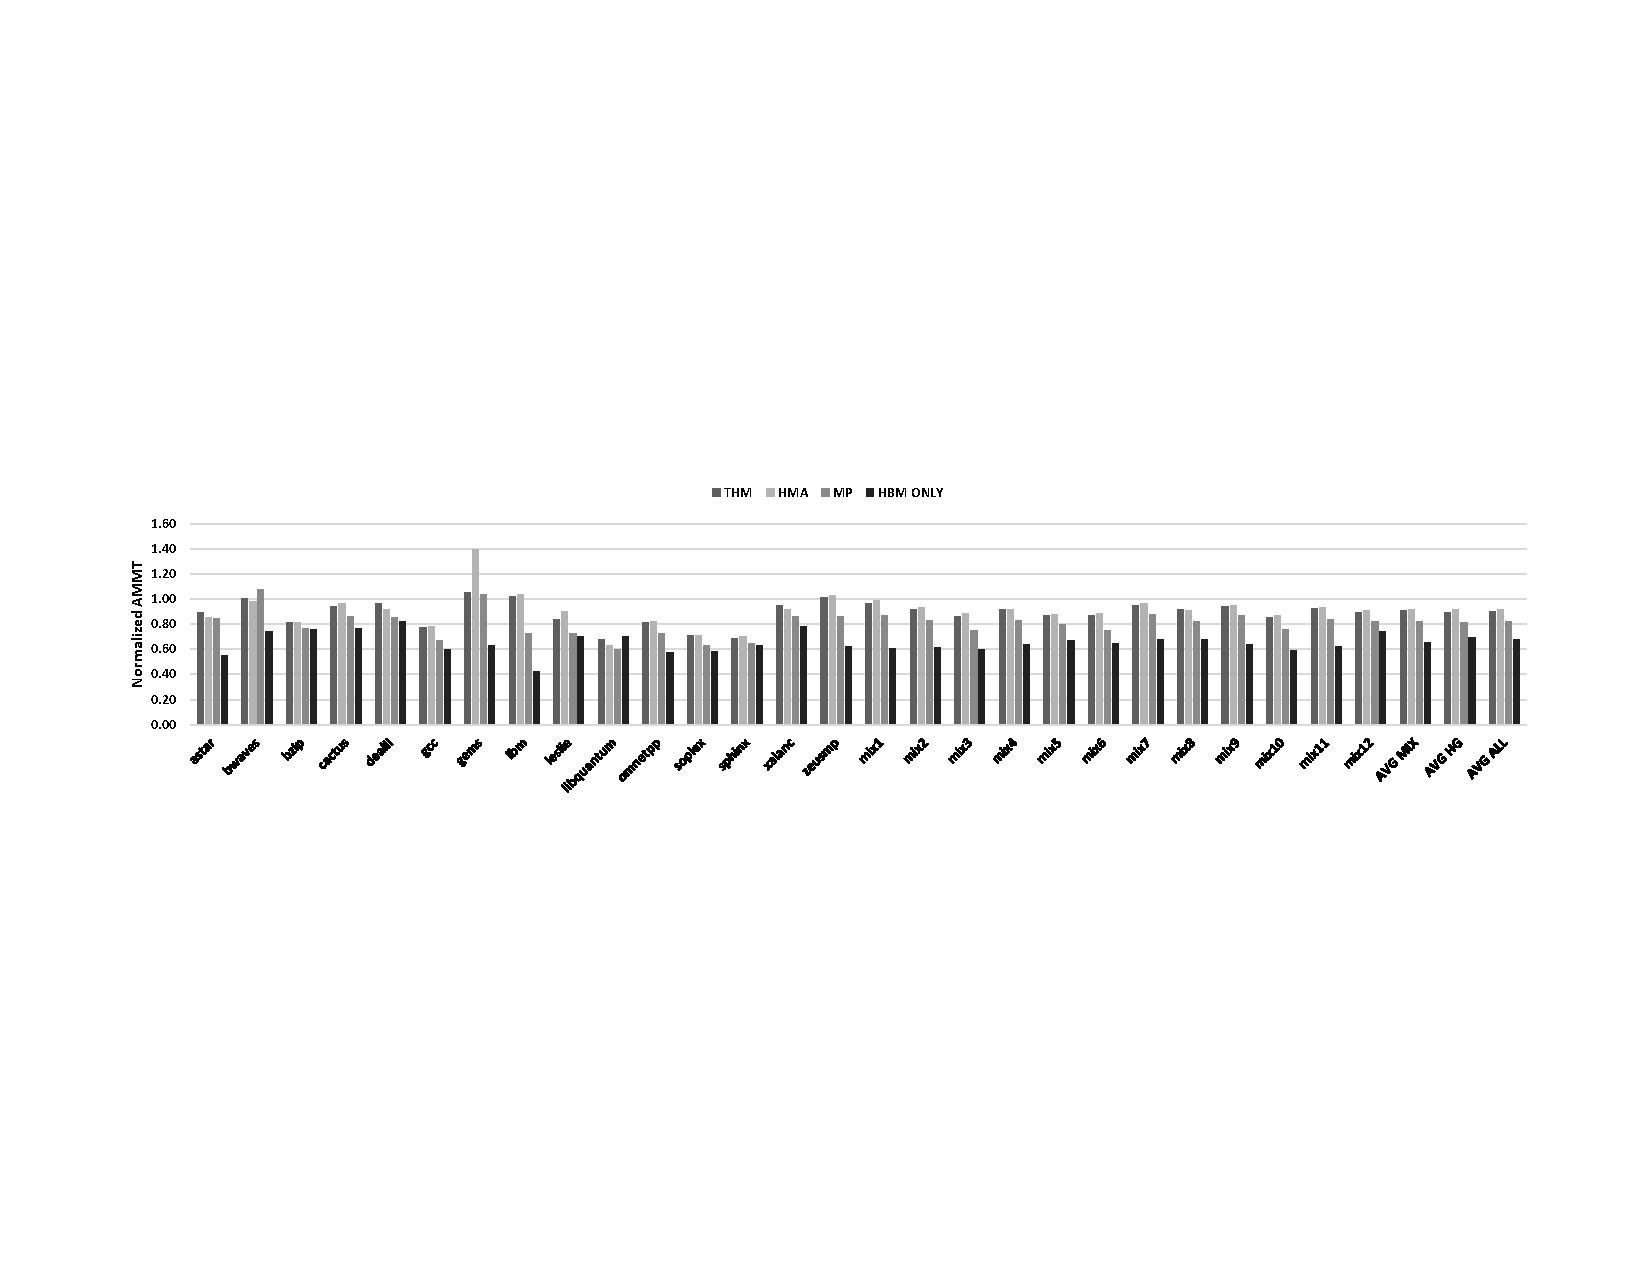
\includegraphics[width=\textwidth]{figures/performance_over_nlm.pdf}
  \caption{Performance Comparison: AMMT is normalized to a hybrid memory without any migration mechanism.}
  \label{fig:performance}
\end{figure*}

Figure \ref{fig:performance} presents a performance comparison of MemPod, HMA, THM and a configuration with 9GBs of on-chip HBM memory, normalized to the performance of a hybrid memory configuration without migration capabilities. We evaluated all mechanisms with caching disabled. 

Based on the results we can derive some interesting observations:
\begin{itemize}[leftmargin=0.4cm]
\setlength\itemsep{0em}
	\item In some workloads migration is harmful to performance, as observed with the bwaves workload, where a no-migration scheme reports higher performance (lower AMMT). We observe that in those cases, MemPod leads to deteriorated performance compared to THM. However, in the case of zeusmp, MemPod increases performance, while THM and HMA report higher AMMT than the no-migration scheme.
	\item MemPod outperforms the state-of-the-art competitors in the majority of our workloads, and in several cases scoring very close to an HBM2-only configuration. 
	\item On average MemPod reports 25\% higher AMMT than HBM2-only, while THM and HMA report 39\% and 41\% respectively.
	\item All mechanisms outperform HBM2-only when executing the libquantum experiment. We attribute this result to a combination of correct timing, application behavior and workload size. In the case of libquantum, to working set size fits entirely in our fast memory. As a results after some migrations, the entire working set will be present in our HBM. However, correct timing is the driving factor behind this impressive performance increase. Our results show the row-buffer hit ratio to be ??x times larger than having HBM2-only (and random page assignment). Apparently, page migrations resulted in an in-memory page order that exploits almost every bit of memory parallelism from the application. This result could be further explored and intentionally recreated in some future work.
\end{itemize}

\subsubsection{Caching Effect}

\begin{figure}
  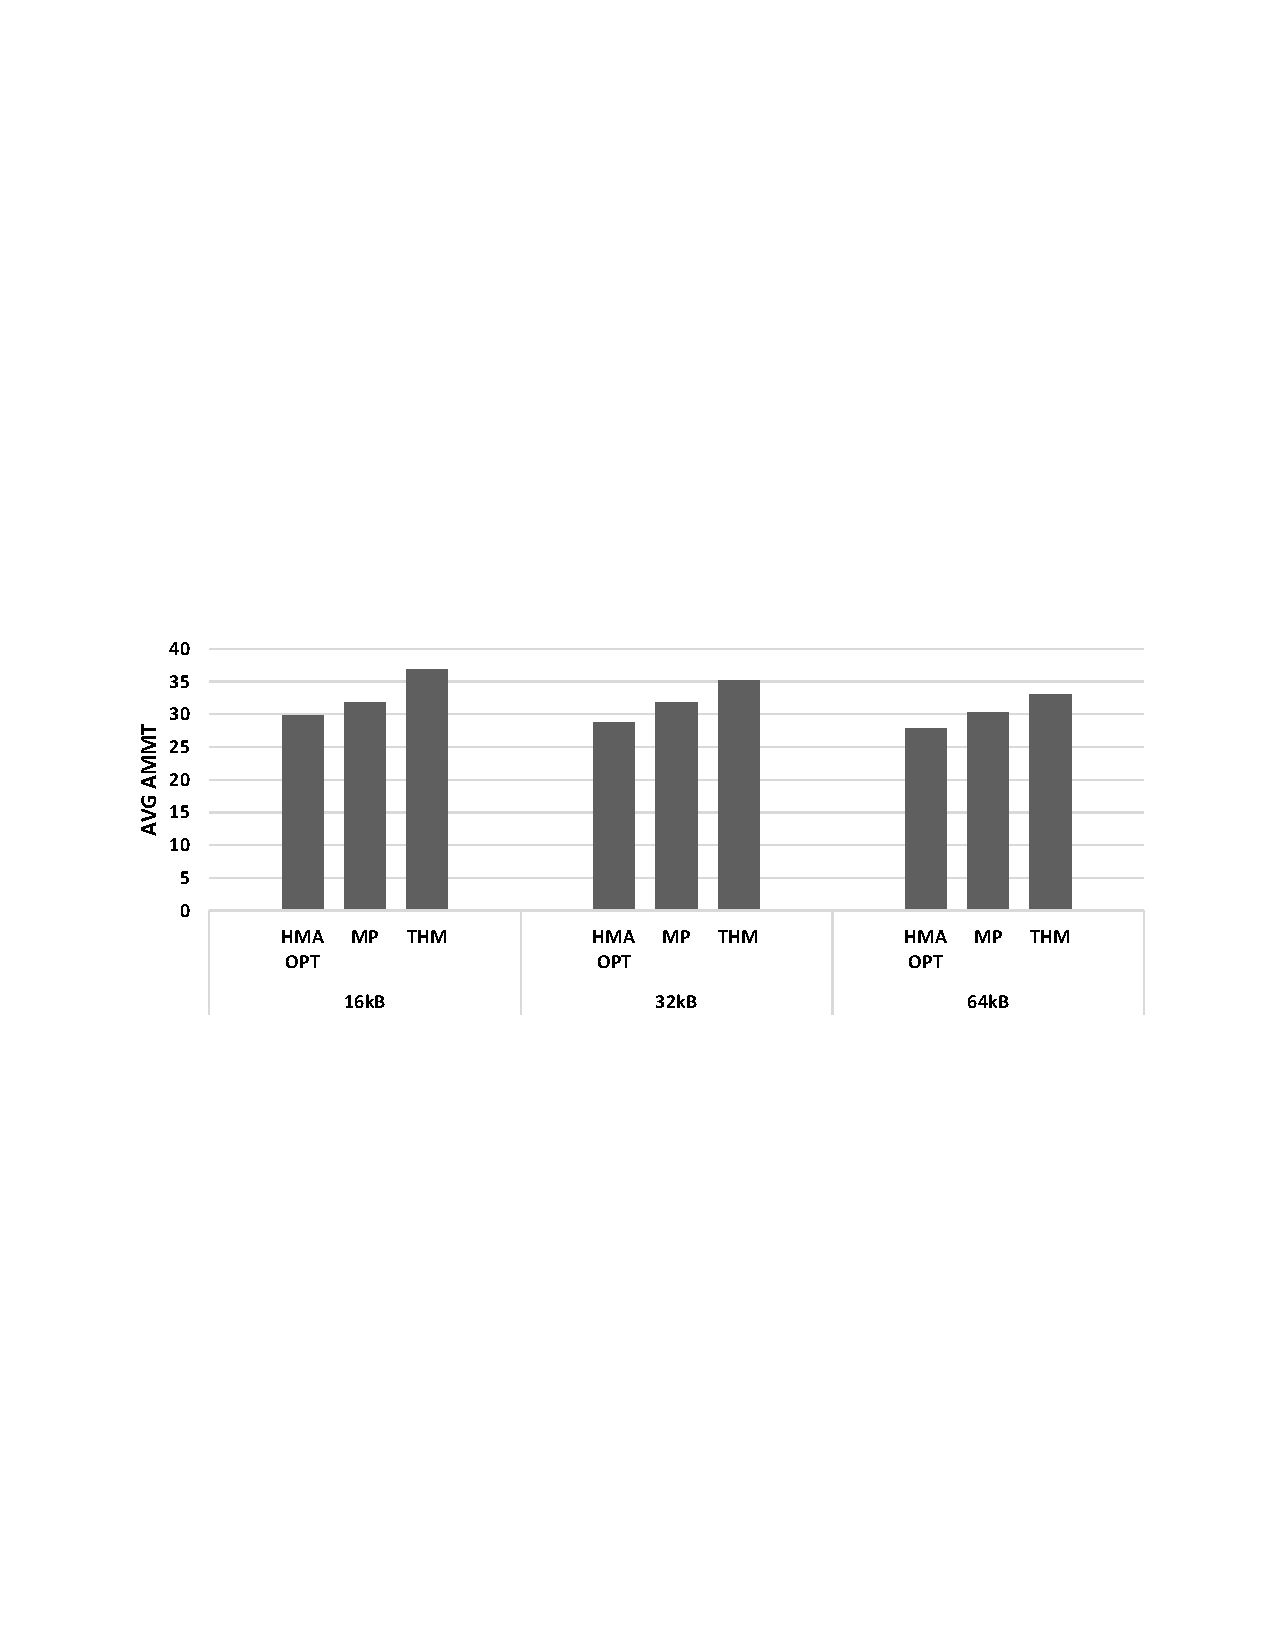
\includegraphics[width=0.46\textwidth]{figures/cache_impact.pdf}
  \caption{Cache Impact}
  \label{fig:cache}
\end{figure}

Migration mechanisms will be forced to include a cache since activity tracking and remap table structures are too large to store on-chip. The use of a cache will unavoidably hinder performance. In this experiment we evaluate the impact of a cache on each mechanism's performance. As described in Section \ref{sec:Architecture}, each mechanism has different cache requirements. THM caches its counters and remap table together with its ``Segmented Remap Table'' structure. HMA has no need for a remap table however it has high storage requirements for its counting mechanism. MemPod must cache its large remap table since MEA counters will be on chip. We simulated each mechanism with 16, 32 and 64 KB of cache. For MemPod, the available cache capacity was divided equally over four Pods. All mechanisms use the stacked memory as backing store.

HMA's design further complicates this study, since sorting all activity counters at each epoch is performed by the OS, utilizing the cpu's cache instead of the dedicated migration cache. In our results, we present ``HMA-OPT'', an HMA flavor that does not take into account any penalties for OS interrupts, TLB shootdowns or Page Table (PT) updates, walks and misses. Even though sorting all HMA's counters will be a costly procedure, in this experiment we assume a ``best-case scenario'' where the entire sorting process is overlapped by requests being serviced from the memory and we don't penalize HMA for sorting. We also do not model the application-level effects of starting with a cold TLB after each interval.

Figure \ref{fig:cache} shows our results obtained by taking the average AMMT from all our workloads for each mechanism. HMA-OPT reports the lowest AMMT, albeit unrealistic and MemPod outperforms every other mechanism regardless of the cache size. MemPod outperforms THM by 9\% a 64kB cache, while HMA-OPT outperforms MemPod by 9\%.

\subsubsection{Scalability}

\begin{figure}
  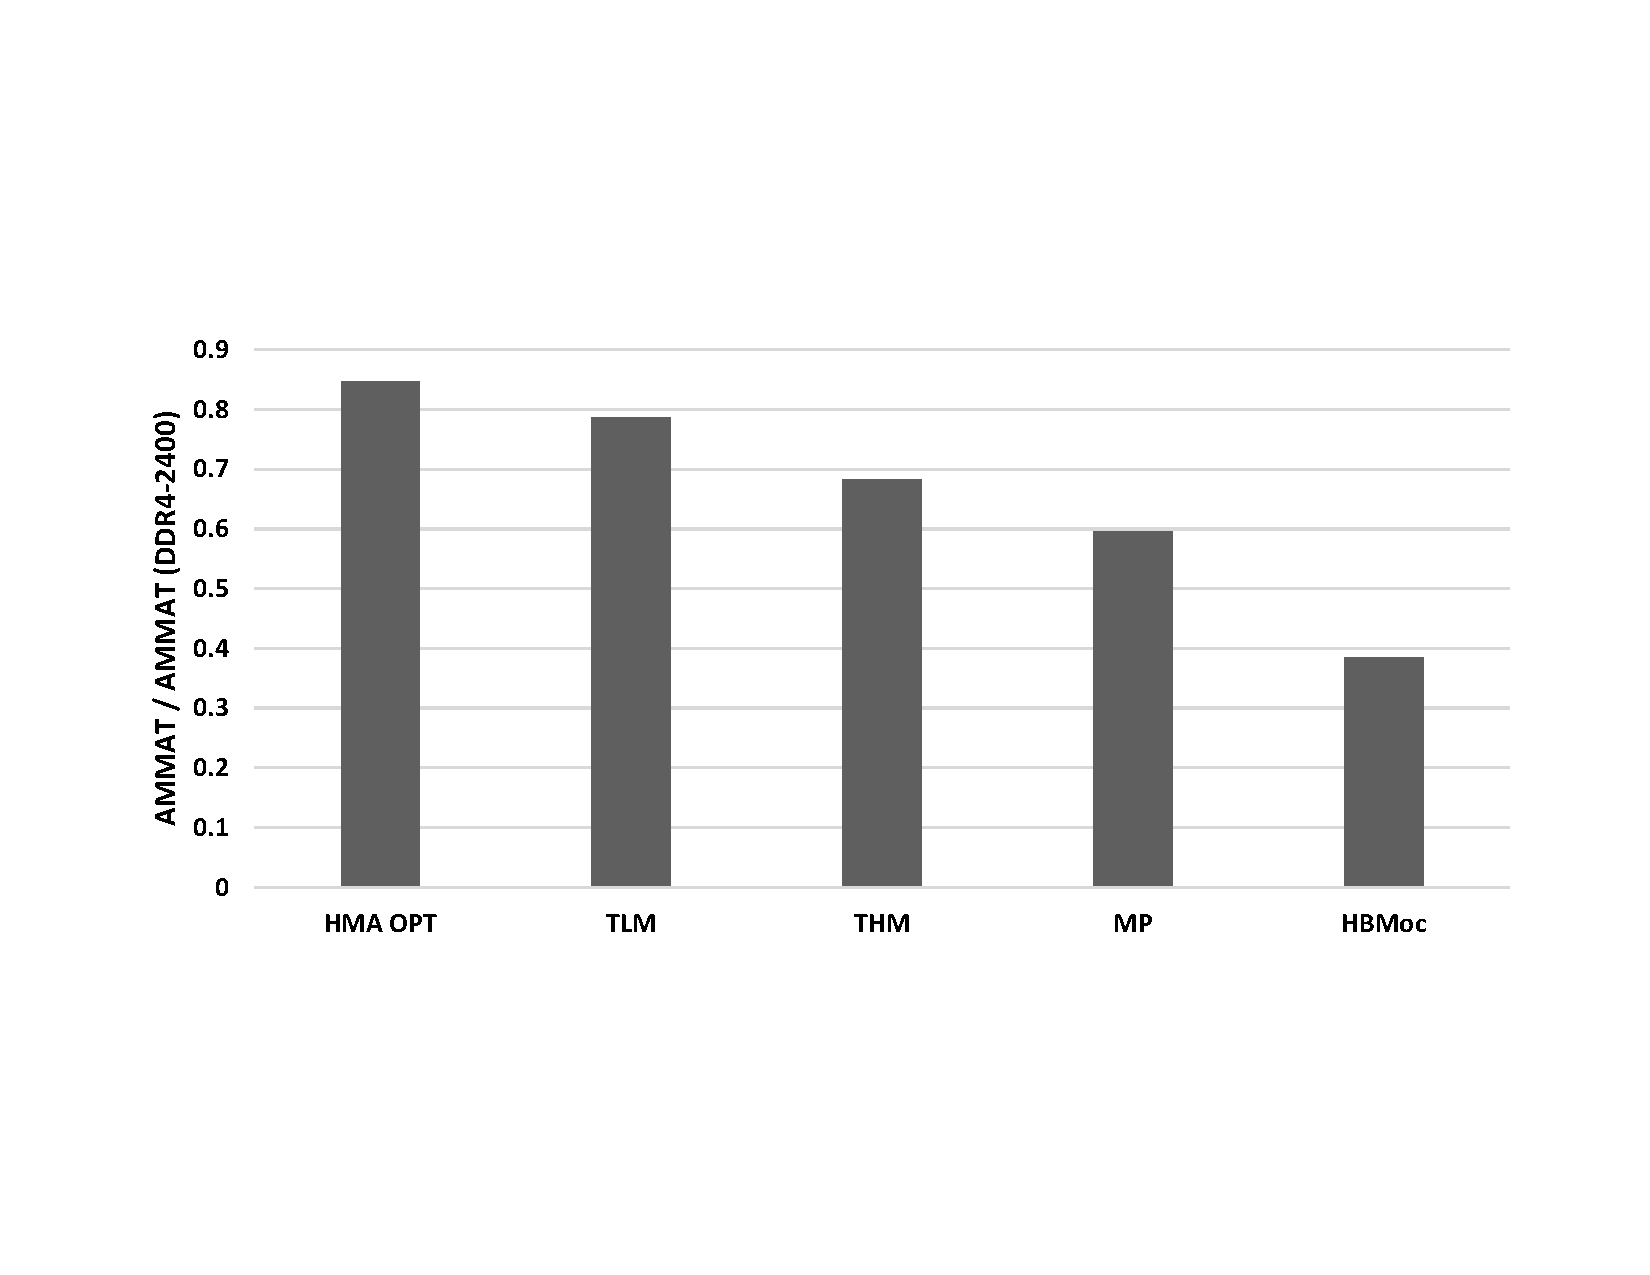
\includegraphics[width=0.46\textwidth]{figures/scalability.pdf}
  \caption{Scalability to faster memories}
  \label{fig:scalability}
\end{figure}

We simulated all mechanism under an overclocked memory configuration in order to evaluate how each one scales with memory technology advances. For this experiment, we used a 4GHz HBM as our stacked memory and a DDR4-2400 as our off-chip memory. Figure \ref{fig:scalability} shows our average AMMT results. The bar labeled ``DDR4-2400'' shows the results from a 9GB configuration with off-chip DDR4 memory only and ``HBMoc'' shows a 9GB configuration with overclocked HBM only. We first observe that HMA-OPT (no penalties added for TLB shootdowns, Page Table updates, sorting counters or OS interrupt) due to its high number of migrations and low prediction accuracy increases AMMT by 8\% compared to a Two-Level Memory without migration (TLM). THM and MemPod reduce AMMT by 13\% and 24\% respectively, compared to TLM. With memory configuration, MemPod reports AMMT improvements of 42\% over HMA-OPT, and 15\% over THM. Compared to the results obtained with a non-overclocked memory, HMA demostrated the worse scalability, improving its average AMMT by 18\%. TLM was improved by 30.5\%, THM by 33\% and MemPod by 35\%.